\documentclass{article}
\usepackage[utf8]{inputenc}
\usepackage[margin = 0.8in]{geometry}
\usepackage{graphicx}
\usepackage{amsmath, amssymb}
\usepackage{subcaption}
\usepackage{multirow}
\usepackage{mathtools}
\usepackage{float}
\usepackage{enumitem}

\DeclareMathOperator*{\wrote}{Wrote}
\DeclareMathOperator*{\copyof}{CopyOf}
\DeclareMathOperator*{\owns2}{Owns}
\DeclareMathOperator*{\sings}{Sings}


\title{CS534 - HW 1}
\author{Keith Chester}
\date{Due date: June 12 2022}

\begin{document}
\maketitle

\section*{Problem 1}

In problem 1, we are tasked with creating a recursive and linear time agent for following propositonal logic statements. The work associated with this problem can be found in \textit{problem1.py}.

\section*{Problem 2}

In this problem we are exploring a first-order logical knowledge base and writing out logical expressions utilizing it. The knowledge base is represented as:

\begin{itemize}
    \item $\copyof(d, a)$ - Predicate - Disk $d$ is a copy of album $a$
    \item $\owns2(p, d)$ - Predicate - Person $p$ owns disk $d$
    \item $\sings(p, s, a)$ - Predicate - Album $a$ inludes a recording of song $s$ sung by person $p$
    \item $\wrote(p, s)$ - Person $p$ wrote song $s$

\end{itemize}

We are also injecting the following constants:
\begin{itemize}
    \item $McCartney$ - a person
    \item $Gershwin$ - a person
    \item $BHoliday$ - a person
    \item $Joe$ - a person
    \item $EleanorRigby$ - a song
    \item $TheManILove$ - a song
    \item $Revolver$ - an album
\end{itemize}

\noindent Within this, we express the following statements using first-order logic:

\begin{enumerate}[label=(\alph*)]
    \item $\wrote(Gershwin, TheManILove)$ %a
    \item $\neg \wrote(Gershwin, EleanorRigby)$ %b
    \item $\wrote(Gershwin, TheManILove) \lor \wrote(McCartney, TheManILove)$ %c
    \item $\exists s \wrote(Joe, s)$ %d
    \item $\exists d \owns2(Joe, CopyOf(d, Revolver))$
    \item $\forall s \sings(McCartney, s, Revolver) \Rightarrow \wrote(McCartney, s)$ %f
    \item $\forall s \sings(p, s, Revolver) \neg \wrote(Gershwin, s)$ %g
    \item $\forall s \wrote(Gershwin, s) \Rightarrow \sings(p, s, a)$ %h
    \item $\exists a \forall s \sings(p, s, a) \wrote(Joe, s)$ %i
    \item $\exists d, a \owns2(Joe, \copyof(d, a)) \land \sings(BHoliday, s, a)$ %j
    \item $\exists d_i \copyof(d_i, a) \forall a \sings(McCartney, a, s) \land \forall  \owns2(Joe, d)$ %k
    \item $\exists d \copyof(d, a) \forall a \sings(BHoliday, s, a) \land \owns2(Joe, d)$ %l
\end{enumerate}

\section*{Problem 3}

In this queston, we are looking at the following table of three binary input atributes, and a singular binary output:

\begin{center}
    \begin{tabular}{ c r r r r }
        Example & $A_1$ & $A_2$ & $A_3$ & Output $y$\\ 
        $x_1$ & $1$ & $0$ & $0$ & $0$\\
        $x_2$ & $1$ & $0$ & $1$ & $0$\\
        $x_3$ & $0$ & $1$ & $0$ & $0$\\
        $x_4$ & $1$ & $1$ & $1$ & $1$\\
        $x_5$ & $1$ & $1$ & $0$ & $1$\\
    \end{tabular}
\end{center}

\subsection*{a.}

Using the Gini Index, we aim to create a decision tree for this data.

\subsection*{b.}

Now we utilize Information Gain to create a decision tree for this data.

\section*{Problem 4}

In this section, we consider the following dta input with six inputs and a singular target output:

\begin{center}
    \begin{tabular}{c r r r r r r r r r r r r r r}
        Example & $A_1$ & $A_2$ & $A_3$ & $A_4$ & $A_5$ & $A_6$ & $A_7$ & $A_8$ & $A_9$ & $A_10$ & $A_11$ & $A_12$ & $A_13$ & $A_14$ \\
        $x_1$ & 1 & 1 & 1 & 1 & 1 & 1 & 1 & 0 & 0 & 0 & 0 & 0 & 0 & 0 \\
        $x_2$ & 0 & 0 & 0 & 1 & 1 & 0 & 0 & 1 & 1 & 0 & 1 & 0 & 1 & 1 \\
        $x_3$ & 1 & 1 & 1 & 0 & 1 & 0 & 0 & 1 & 1 & 0 & 0 & 0 & 1 & 1 \\
        $x_4$ & 0 & 1 & 0 & 0 & 1 & 0 & 0 & 1 & 0 & 1 & 1 & 1 & 0 & 1 \\
        $x_5$ & 0 & 0 & 1 & 1 & 0 & 1 & 1 & 0 & 1 & 1 & 0 & 0 & 1 & 0 \\
        $x_6$ & 0 & 0 & 0 & 1 & 0 & 1 & 0 & 1 & 1 & 0 & 1 & 1 & 1 & 0 \\
        $T$ & 1 & 1 & 1 & 1 & 1 & 1 & 0 & 1 & 0 & 0 & 0 & 0 & 0 & 0 \\

    \end{tabular}
\end{center}

When we run our code found in \textit{problem4.py}, we find that we can train both a perceptron and decision tree on this data. If given unseen data of $A_{15}:<1, 1, 0, 0, 1, 1>$ with result $T_{15}=1$, we find that both accurately predict this result.

Whne we generate the decision tree, we can output its resulting branches, seen as follows:

\begin{figure}[H]
    \centering
    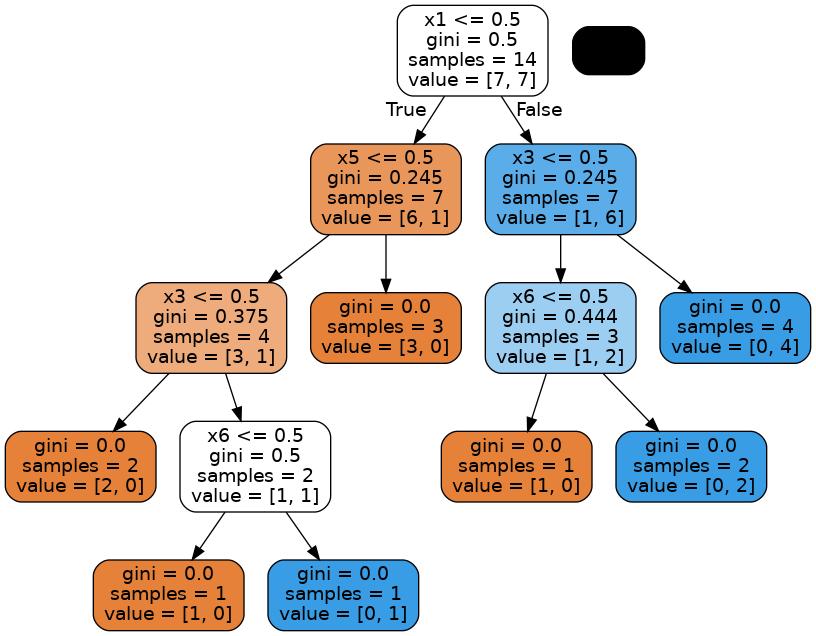
\includegraphics[width = 0.65\textwidth]{tree.png}
\end{figure}

Our code that utilizes the perceptron makes a perceptron makes a perceptron enacting the following linear equation:

\begin{equation}
    T = 6x_1 + 0x_2 + 3x_3 - 2x_4 - 4x_5 + 4x_6 - 4
\end{equation}

\end{document}